\chapter{Stars, Bars and Hockey Sticks}
\section{Introduction}
While almost all problems can be solved using the CCC, sometimes its quicker to remember a certain fact. This chapter goes through some facts which should be kept in mind as such configurations occur quite often.
\section{Stars and Bars}
\begin{example}
    [Motivating Example] In how many ways can 10 choclates be divided among 3 children(The children are distinguishable, the choclates aren't)?
\end{example}
\begin{proof}
    [Solution]
    Let's re frame the question as ways to insert two identical dividers in a line of 10 chocolates. We are looking for the permutations of this(Think of why this is exactly the same thing)\\
    The number of such permutations will be: $\frac{(10+2)!}{2!*10!}$\\
    Which is equal to 66.
\end{proof}
Generalizing this: 
\begin{theorem}
[Stars and Bars]
    we can say that n objects can be put in k distinguishable bins in   $\frac{(n+k-1)!}{n!*(k-1)!}=\binom{n+k-1}{n}$
\end{theorem}
The Stars and Bars has various uses
\begin{example}
    Alice has 24 apples. In how many ways can she share them with Becky and Chris so that each of the three people has at least two apples?
\end{example}
\section{Counting in two ways}
While playing the guessing game, you may have found yourself having two or more ways to solve the same question both ,hopefully, leading to the same answer. But as one method is easier to compute than the other, we use that. But if we think about it, given a configuration, we should get the same number of permutation or combination using any method.\\
This idea is what we use. We calculate the same, generalized thing in two ways and equate them to get an identity, which we can use elsewhere as it is true in general.\\
This is called counting in two ways. Let's see it in action:
\begin{example}
    [Motivating Example]
    How many councils with at least 1 member and at most n members be made from a pool of n people?
\end{example}
\begin{proof}
    [Solution]
    We obviously know that the answer is $2^n - 1$ from the subset theorem. \\
    However we can also write this as $\binom{n}{1} + \binom{n}{2} \dots \binom{n}{n}$\\
    We can, hence say, $\binom{n}{1} + \binom{n}{2} \dots \binom{n}{n}= 2^n -1$ \\
    $\therefore \binom{n}{1} + \binom{n}{2} \dots \binom{n}{n} +1 = 2^n$ \\
    as we know $\binom{n}{0}=1$, we can say: $\binom{n}{0} + \binom{n}{1} + \binom{n}{2} \dots \binom{n}{n} = 2^n$
\end{proof}
What we just derived is called the Binomial identity.
\begin{theorem}
    $\binom{n}{0} + \binom{n}{1} + \binom{n}{2} \dots \binom{n}{n} = 2^n$
\end{theorem}
This is surprisingly useful even in algebra.\\
\begin{example}
    [Motivating Example]
     Suppose a committee consists of m men and n women. In how many ways can a subcommittee of r members be formed?
\end{example}
\begin{proof}
    [Solution]
    We obviously know that the answer is $\binom{m+n}{r}$ from the subset theorem. \\
    However we can also write this as $\binom{m}{0}*\binom{n}{r-0} + \binom{m}{1}*\binom{n}{r-1} \dots +\binom{m}{r-1}*\binom{n}{1}+\binom{m}{r}*\binom{n}{0}$\\
    We can, hence say, $\binom{m}{0}*\binom{n}{r-0} + \binom{m}{1}*\binom{n}{r-1} \dots +\binom{m}{r-1}*\binom{n}{1}+\binom{m}{r}*\binom{n}{0}=\binom{m+n}{r}$ \\
    \end{proof}
This is called Vandermonde’s Identity.
\begin{theorem}
    $\binom{m}{0}*\binom{n}{r-0} + \binom{m}{1}*\binom{n}{r-1} \dots +\binom{m}{r-1}*\binom{n}{1}+\binom{m}{r}*\binom{n}{0}=\binom{m+n}{r}$
\end{theorem}
\section{Pascal's Triangle}
\begin{figure}[H]
    \centering
    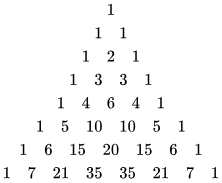
\includegraphics[width=0.75\linewidth]{Photos/pascal triangle.png}
    \caption{Enter Caption}
    \label{fig:enter-label}
\end{figure}
The triangle somewhere on the top of the page is called Pascal's triangle. \\
It has a lot of fun and amazing properties(try to find them, you'll be surprised).\\
We are going to exploit two of them right now. First being, Every term in subsequent line is made by adding the two above it. The second being that it can be written as follows:
\begin{figure}[H]
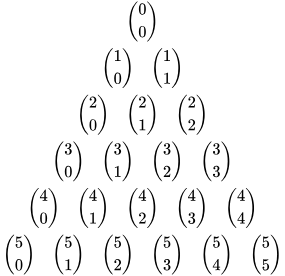
\includegraphics{Photos/Binomial Pascal.png}
\end{figure}
This is exceptionally useful as this leads us to Pascal's Identity
\begin{theorem}
    $\binom{n}{k} + \binom{n}{k+1}=\binom{n+1}{k+1}$
\end{theorem}
and the hockey stick identity(try looking at a diagonal)
\begin{theorem}
    $\binom{k}{k}+\binom{k+1}{k}+ \dots +\binom{n}{k}=\binom{n+1}{k+1}$
\end{theorem}
These identities can be memorized quite simply by writing them on a piece of paper and taping them to a wall next to where you sleep. Every morning look at it just after you wake up, and every night just before you sleep. You'll have them memorized in less then a week.\\
The another way to remember the is by simply solving the questions and deriving every identity you forget, no turning the pages back. That will get it done in less than  two hours flat.\\
Solve at least questions worth \points{60}. This exercise has a total of \points{75}.
\begin{xcb}{Exercises}
\begin{enumerate}
\item \points{2} In how many ways can one get $10$ upon rolling $7$ dice?
\item \points{2} How many $4$ digit numbers have a sum of $9$?
\item \points{3} How many ordered pairs $(a,b,c,d)$ where $a \le b \le c \le d \le 5$ and $a,b,c,d \in \mathbb{N}$?
\begin{hint}
    \addhint{Let $a=1+x$, $b=a+y$ and so on. Does this look like a Stars and Bars now?}
\end{hint}
\item (AIME 2000) \points{9} Given that\\
\[\frac 1{2!17!}+\frac 1{3!16!}+\frac 1{4!15!}+\frac 1{5!14!}+\frac 1{6!13!}+\frac 1{7!12!}+\frac 1{8!11!}+\frac 1{9!10!}=\frac N{1!18!}\]
find the greatest integer that is less than $\frac N{100}$.
\begin{hint}
    \addhint{Multiply both sides by $19!$}\\
    \addhint{Multiply both sides by $2$ and use $\binom{n}{k}=\binom{n}{n-k}$}
    \addhint{Add terms to reach an identity which we know the summation to}
\end{hint}
\item(AIME 2001) \points{3} A fair die is rolled four times. The probability that each of the final three rolls is at least as large as the roll preceding it may be expressed in the form $m/n$ where m and n are relatively prime positive integers. Find $m + n$.
\item (AMC 8 2018) \points{3} From a regular octagon, a triangle is formed by connecting three randomly chosen vertices of the octagon. What is the probability that at least one of the sides of the triangle is also a side of the octagon?
\begin{hint}
    \addhint{Can we convert the choosing of $3$ points as partitioning of remaining $5$ points into $3$?}
\end{hint}
\item(AIME 2020) \points{2} A club consisting of $11$ men and $12$ women needs to choose a committee from among its members so that the number of women on the committee is one more than the number of men on the committee. The committee could have as few as $1$ member or as many as $23$ members. Let $N$ be the number of such committees that can be formed. If $N=\binom{a}{b}$, find $a + b$
\begin{hint}
    \addhint{We'll use Vandermonde identity, now try to solve it.}
\end{hint}
\item (AIME 2015) \points{3} Consider all 1000-element subsets of the set ${{1, 2, 3, \dots , 2015}}$. From each such subset choose the least element. The arithmetic mean of all of these least elements is $p/q$, where $p$ and $q$ are relatively prime positive integers. Find $p + q$.
\begin{hint}
    \addhint{$a_1+2a_2+3a_3+\dots na_n=(a_1+a_2+\dots+a_n)+(a_2+a_3+\dots)+\dots+(a_n)$}
\end{hint}
\item \points{2} For how many positive integers $x_1, x_2, \dots, x_{10}$ do we have $x_1 + x_2 + \dots + x_{10} = 50$?
\item (AIME 2011) \points{5} Ed has five identical green marbles, and a large supply of identical red marbles. He arranges the green marbles and some of the red ones in a row and finds that the number of marbles whose right hand neighbor is the same color as themselves is equal to the number of marbles whose right hand neighbor is the other color. An example of such an arrangement is $GGRRRGGRG$. Let $m$ be the maximum number of red marbles for which such an arrangement is possible, and let $N$ be the number of ways he can arrange the $m+5$ marbles to satisfy the requirement. Find the remainder when $N$ is divided by $1000$.
\begin{hint}
    \addhint{$m$ is limited by the fact that number of marbles whose right hand neighbor is the other color is maximum 10. How many red marbles will we need for this to lead to a valid arrangement?}
    \addhint{As we know $m$ now, can we simply use stars and bars with one red marble always between 2 green.}
\end{hint}
\item (AIME 2011) \points{9} Six men and some number of women stand in a line in random order. Let $p$ be the probability that a group of at least four men stand together in the line, given that every man stands next to at least one other man. Find the least number of women in the line such that $p$ does not exceed 1 percent.
\begin{hint}
    \addhint{In what ways can the men be arranged in? Use the groups of men as bars and the women as stars}
    \addhint{Use Pascal to simplify and then open the binomial}
\end{hint}
\item \points{2} Let $n$ be a positive integer. In how many ways can one write a sum of at least two positive integers that add up to $n$?
\item (AIME 2013) \points{5} Melinda has three empty boxes and $12$ textbooks, three of which are mathematics textbooks. One box will hold any three of her textbooks, one will hold any four of her textbooks, and one will hold any five of her textbooks. If Melinda packs her textbooks into these boxes in random order, the probability that all three mathematics textbooks end up in the same box can be written as $\frac{m}{n}$, where $m$ and $n$ are relatively prime positive integers. Find $m+n$.
\begin{hint}
    \addhint{Casework onto the box in which the three math textbooks are in}
    \addhint{Simplify before you compute! Take $9!$ common, multiply numerator and denominator by $3!4!5!$}
\end{hint}
\item (AMC 10 2016) \points{3} For some particular value of $N$, when $(a + b + c + d + 1)^N$ is expanded and like terms are combined, the resulting expression contains exactly $1001$ terms that include all four variables $a, b, c,$ and $d$, each to some positive power. What is $N$?
\item (AMC 12 2021) \points{9} A choir director must select a group of singers from among his $6$ tenors and $8$ basses. The only requirements are that the difference between the number of tenors and basses must be a multiple of $4$, and the group must have at least one singer. Let $N$ be the number of different groups that could be selected. What is the remainder when $N$ is divided by $100$?
\begin{hint}
    \addhint{Casework on the tenors $-$ basses combined with Vandermonde will work.}
\end{hint}
\item (IMO 1981/2) \points{9} Let $\displaystyle 1 \le r \le n$ and consider all subsets of $\displaystyle r$ elements of the set $\{ 1, 2, \ldots , n \}$. Each of these subsets has a smallest member. Let $\displaystyle F(n,r)$ denote the arithmetic mean of these smallest numbers; prove that\\
\[F(n,r) = \frac{n+1}{r+1}.\]
\begin{hint}
    \addhint{We have already solved a case of it as an AIME 2015 problem, won't the same technique work in general?}
\end{hint}
\item \points{5} Prove that \[\sum_{k=0}^n k{\binom{n}{k}}^2=n\binom{2n-1}{n-1}\]
\end{enumerate}
\end{xcb}